
\subsubsection{Twirling}

It is not the fact that the success probabilities are lower for odd parities than for even parity that is especially concerning; this is what fault-tolerant codes are designed to cope with. Instead it is the fact that bit-flips on each qubit give a \emph{different} probability of successful detection. This means one qubit will me more prone to undetected errors than others. The fault tolerance required by the proposal assumes a symmetry between the data qubits that this breaks, making the code susceptible to logical errors.

A method proposed to account for this is suggested in the proposal \cite{OGorman2016}. Their \emph{`twirling'} technique smooths out this asymmetry between data qubits by effectively switching the location of bit-flips randomly so that the phase accumulated due to any one bit-flip is on average the same as for any other bit-flip. This is done by randomly applying one of four unitary operations $\mathrm{U_1 = \op{I}\op{I}\op{I}\op{I}}$, $\mathrm{U_2 = \op{I}\op{I}\op{X}\op{X}}$, $\mathrm{U_3 = \op{I}\op{X}\op{I}\op{X}}$, $\mathrm{U_4 = \op{I}\op{X}\op{X}\op{I}}$, as illustrated in fig. \ref{fig:twirls}, both before and after the parity measurement.

This has the effect of making the average projection onto the $x$-axis the same for all odd parity cases as desired, at the expense of reduced success probability for even parity. This risks introducing Pauli errors \cite{OGorman2016} but provided the success probability is sufficiently high this is correctable by the code.


\begin{figure}
	\centering
	%	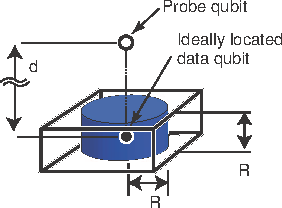
\includegraphics[width=\columnwidth]{../Figures/pillbox.pdf}
	\subfloat[]{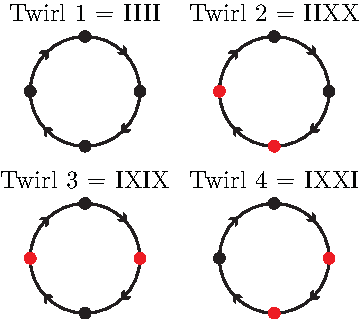
\includegraphics[width=0.4\columnwidth]{../Figures/twirls.pdf} \label{fig:twirls}}
	\subfloat[]{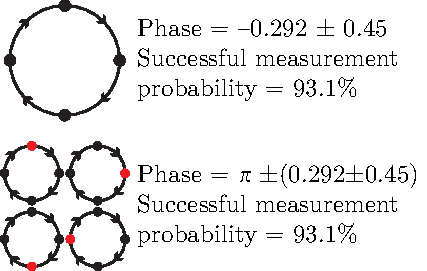
\includegraphics[width=0.5\columnwidth]{../Figures/twirl_effect.pdf} \label{fig:twirleffect}}
	\caption{`Twirling' operations. (a) Each of the four twirling operations which, when applied with equal probability, randomly change which qubit effectively contributes to odd parity, smoothing out asymmetries in success probabilities due to qubit displacements. (b) Effect on success probabilities for the displacements shown in fig.\@ \ref{fig:qubitdisplacements}. Even parity shows a reduction in success probability, while the success of odd parity measurements becomes constant on average.}
\end{figure}